\documentclass[11pt]{article}
\setlength{\textwidth}{6.3in}
\setlength{\textheight}{9in}
\setlength{\oddsidemargin}{0in}
\setlength{\evensidemargin}{0in}
\setlength{\topmargin}{-.6in}
\linespread{1.3}

% \renewcommand{\labelenumi}{\alph{enumi}}
\usepackage{epsfig}
\usepackage{amsmath}
\usepackage{amssymb}
\usepackage{amsfonts}
\usepackage{tikz}
\newcommand{\spacer}{\displaystyle{\phantom{\int}}}
\newcommand{\blank}[1]{\underline{\hspace{#1}}}
\newenvironment{piecewise}{\left\{\begin{array}{l@{,\quad}l}}{\end{array}\right.}
\newcommand{\points}[1]{({\it #1 points})}
\hyphenation{}

\graphicspath{ {./}{../figures/} }

\begin{document}
\noindent \textbf{Sam Voisin \hfill  \textbf{Topological Data Analysis: Class Project}  \hfill  December 11, 2019} \\
\line(1,0){455}

\begin{center}
\Large{{\bf Gesture Recognition via Electromyograph Signals}}\\
\end{center}

\begin{enumerate}
\setlength{\parindent}{5ex}

\item \textbf{Introduction}

\noindent

Skeletal muscles produce electrical activity known as \emph{myoelectric impulses} upon contraction. These myoelectric impulses can be detected and recorded using an electromyograph (EMG). EMGs are currently used to study a number of neuromuscular conditions.

Two electromyograph categories exist currently. The first type of EMG, introduced in 1950, is the \emph{intramuscular EMG}. The intramuscular EMG uses subcutaneous sensors implanted in the skeletal muscle through thin wires. The second EMG type is the \emph{Surface} electromyograph ("sEMG"). The sEMG uses sets of two or more electrodes placed on the surface of the skin. The sEMG  represents a compromise between the invasive nature and greater precision associated with its intramuscular counterpart. 

Superficial qualities of the subject being measured can have a detrimental affect on the quality of sensor readings. Some examples of these qualities are perspiration, body-fat content, or shifting of sensor pads \cite{lobov}.

A more recent technology trend is that of wearable technology or \emph{wearables} \cite{wear}. Modern wearables typically perform a variety of tasks including providing information such as text message alerts and capturing biological data such as the user's heart rate. Wearables have been depicted in SciFi novels and movies for decades but have only recently become common to consumers. As discussed in section 3, quality wearable devices combined with reliable and cost-effective myoelectric sensing technology may lead to a new generation of intuitive human-computer interface ("HCI") devices.

\item \textbf{Problem Statement}

As sEMG devices decline in size and cost, they have become a focus for researchers interested in the information they might provide.The problem of classifying motion as captured with sEMG sensors is not a new one. Researchers have published articles as early as 1967. Indeed, the number of publications on the topic has grown considerably in the last 20 years \cite{state}. In particular, the problem of classifying movements is now popular enough that several datasets of recorded signals and subject characteristics have been generated and published \cite{ninapro}.

As stated above, there have been many successful attempts to classify gestures  using EMG sensor data. Common methods employed to this task are linear discriminant analysis, artificial neural networks, support-vector machines and more \cite{state}. Despite this success, consumers have been slow to adopt HCI devices for a number of reasons. Two major factors represent hurdles to continued advances in this area:
\begin{enumerate}
\item[1)] Limited computational resources - Available processing power and on-board memory are restricted to what can be embedded in a necessarily low-profile device. The artificial neural network ("ANN") is a prime example of a high-performing algorithm that has performed will in-sample but does not generalize well due to these constraints.

\item[2)] Availability of training data - The amount of training data required to achieve satisfactory results without overfitting is limited to the quality and configuration of equipment of a single study \cite{bigdata}. While the NinaPro database offers a number of relevant data to be used in training gestures classifiers, the data is generated across differing experiments where test subjects make differing gestures while wearing sensor arrays in differing configurations. As a result, the amount of available training data is not linear in the number of new studies being performed.
\end{enumerate}

This project seeks determine whether it is possible to identify latent features common to various classes of gestures while removing variance associated with superficial qualities of the test subject and minor differences in quality and configuration of the sEMG sensor array. The figure 1 depicts a proposed data pipeline for this purpose.

\begin{figure}[h]
\centering
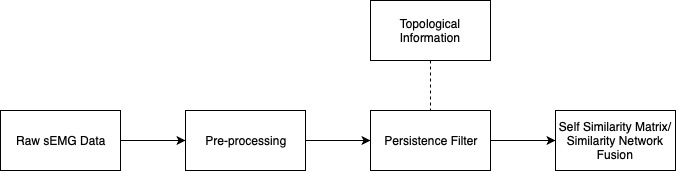
\includegraphics[width=0.5\textwidth]{pipeline}
\caption{Proposed data pipeline}
\end{figure}

This pipeline consists of two primary components:
\begin{enumerate}
\item A filtering component capable of remove superficial noise inessential to classifying gestures.
\item A classification component capable of identifying a gesture. Ideally this classification will be performed as early as possible in the gesture cycle.
\end{enumerate}
Hypotheses, testing, and construction of these components are described in greater detail in section 4. If the suggested pipeline is feasible, training data captured across studies may be utilized in classification with minimal information loss.

\item \textbf{Previous Work}

The primary work that inspired this project is  \emph{Latent Factors Limiting the Performance of sEMG-Interfaces} by Lobov, \emph{et al.} \cite{lobov}. The research team in this study set out to train both a linear discriminant analysis ("LDA") classifier and an artificial neural network ("ANN") classifier capable of identifying gestures. The classifier would then be used to assist users in playing a simple game via the \emph{Myohalmic armband}, a wearable HCI device equipped an sEMG sensor array. Subjects were able to control the game with some success using gestures. However, performance was far better when using a mouse or joystick. The sEMG training data was smoothed using a root mean square (RMS) moving average.

More recently, Phinyomark \emph{et al.} found applications of TDA for EMG data similar to those generated in \cite{Lobov}. They sampled overlapping windows of EMG signals and then reduced the dimension of these windows via principal component analysis. The \emph{mapper} algorithm was applied to the resulting vectors to create a topological network representing the feature space of EMG signals. Signal amplitude and power, nonlinear complexity and frequency information, and time-series structure were determined to be the most influential features for identifying gesture patterns \cite{topograph}.

---

The preferred classifier to be utilized in the pipeline in figure 1 is based on the similarity network fusion ("SNF") described by Traile, Bendich, and Harer in \emph{Multi-Scale Geometric Summaries for Similarity-Based Sensor Fusion} \cite{ssm2} and self-similarity matrices ("SSMs").

SSMs are matrices generated by calculating the value of an appropriate distance metric between all of the points in a discrete time series. A set of SSMs generated from differing signal sources can then be "fused" into a template for unsupervised classification. This approach to clustering seems appropriate to the problem at hand because it was developed to handle sensor data generated from differing sources much like the 8 sensors in my data set (section 3). Additionally, this technique does not need the large, homogeneous training data sets required to adequately fit ANNs or other models with large parameter sets.

\item \textbf{Data}

The data set I will be using for this project is the \emph{EMG data for gestures Data Set} from the UCI Machine Learning Repository \cite{uci}. This data set was collected by Lobov, \emph{et al.} during the study described in the previous section.

This data set consists of 36 subjects performing a series of six distinct gestures. Each subject performed their gestures four times for approximately three seconds per gesture. The motions were captured by a bracelet placed on the forearm and transmitted via Bluetooth to a PC where the data was recorded. The bracelet was equipped with 8 evenly spaced sEMG sensors. The result is a data set of approximately 864 matrices of size $t \times 10$ where $t$ represents elapsed time in milliseconds. The 10 columns of each matrix are time, sensor readings 1 - 8, and a gesture label.

\item \textbf{Analysis Methods \& Pipeline}

My goal is to develop a data pipeline that consists of a component capable of filtering out statistical noise and emphasizing important topological features of a signal and a component capable of classifying a gesture in an unsupervised manner.

Methods from topological data analysis will be utilized for feature extraction. Persistence diagrams allow us to inform decisions about high-dimensional geometric properties of data without the information loss associated with other techniques for visualizing features (e.g. principle component analysis). Persistence images use a weighting function to emphasize pertinent topological features of a signal and de-emphasize noise. This approach should outperform the typical moving average approach \cite{state} to pre-processing sEMG signals which "bake-in" signal noise and in some cases smooth over potentially important characteristics like medium-sized amplitudes.

Important topological characteristics identified in this way will be used to encode a filter capable of differentiating useful signal from statistical noise. This represents the first stage in the pipeline. The filter will work by discarding the irrelevant components of the sEMG modalities as identified in the previous paragraph and keeping those components that provide useful information. For example, this might mean removing all periods whose absolute amplitude is less than some threshold which corresponds to imprecision in the sEMG sensor bracelet.

The next stage of the pipeline will feature a classifier capable of differentiating gestures based on their vectorized persistence diagrams or images. A supervised method will first be utilized here to test the separability of the gesture classes. Following tests of supervised learners and separability of the vectors, unsupervised methods of clustering will be employed. The intention of using unsupervised methods is to further provide evidence that large training samples and complex machine learning algorithms are not strictly necessary for gesture recognition. Currently, the preferred classifier for this stage in my pipeline is the SSM described in section 2 paragraph 3.

\newpage

\item \textbf{Software}

My exploratory work with the data set thus far has utilized Python's standard packages for data analysis including matplotlib and NumPy. Additionally, I have been working with libraries that comprise the Scikit-TDA such as ripser, persim, and cechmate. I have already created a series of specialized functions for performing the analysis and building the pipeline described in the previous section. Looking forward the functions in Scikit-TDA should be sufficient for my needs throughout this project.

The supervised and unsupervised classifiers in the second stage of my pipeline will be implemented via the scikit-learn library. Additional libraries will be employed as needed for these purposes. The SSM approach \cite{ssm1}\cite{ssm2} to unsupervised clustering will likely require that I develop several functions to meet my specific needs. This should be feasible using NumPy and SciPy, but may require some optimization for run-time efficiency. This can likely be performed using a number of Python-based C/ C++ optimization tools. Time permitting, this may also provide an opportunity to develop and employ functions in Julia to take advantage of the high-performance numerical analysis features found there.

\item \textbf{Risk Mitigation}

Current exploratory analysis is promising. However, there are three primary areas which could slow progress:
\begin{enumerate}
\item[1.] \emph{High computational complexity} - As exploratory analysis continue there may come a point where computing various complexes and persistence diagrams becomes computationally infeasible. This scenario is low risk as a significant amount of computation has already been performed without issue. The libraries described in the previous section are well optimized and the data set is not overly complex. Nevertheless, should computation become an issue the code and data can quickly be transferred to Duke's distributed servers and docker containers. Thus development will continue while other components are tested and tasks are performed.
\item[2.] \emph{Poor classifier performance} - This is also low risk. There are many alternative methods for classifying gestures. The real risk in this area is the risk of over-fitting a particular classifier to the data set resulting in poor out-of-sample performance. The goal of the project is to find a classifier that is invariant to the user who is making the gesture. Over-fitting the data would result in a failure to achieve this goal. To prevent over-fitting, I will employ a modified form of k-fold cross validation that will remove all gestures performed by k subjects from the data set. In the case of a supervised algorithm, I will fit the model to the training data and test on the hold out data. This cross validation method can be used to test the quality of unsupervised methods as well. For the unsupervised algorithms, I will generate clusters from the training data and then see how well the hold-out data fits into these clusters via a cluster purity metric or the like.
\item[3.] \emph{Inability to identify important features} - This is the greatest risk to the project goals. Inability to detect latent features in the modalities could be due to a number of factors including data quality, sensor imprecision, etc. If this scenario arises, various transformations will be employed on the data set in an attempt to uncover these features. Should that fail to mitigate the problem, I will explore alternative sEMG data sets.
\end{enumerate}

\end{enumerate}

\begin{center}
\noindent\rule{16cm}{0.4pt}
\end{center}


\begin{thebibliography}{5}

\bibitem{lobov} Lobov, Sergey, et al. “Latent Factors Limiting the Performance of sEMG-Interfaces.” Sensors, vol. 18, no. 4, June 2018, p. 1122., doi:10.3390/s18041122.

\bibitem{wear} Tehrani, Kiana, and Andrew Michael. “Wearable Technology and Wearable Devices: Everything You Need to Know.” Wearable Devices Magazine, WearableDevices.com, March 2014. Web.

\bibitem{state} Peerdeman  B,  Boere  D,  Witteveen  H,  Huis  in  ‘t  Veld  R,  Hermens H, Stramigioli S, Rietman H, Veltink P, Misra S. Myoelectric  forearm  prostheses:  State  of  the  art  from  a  user-centered perspective. J Rehabil Res Dev. 2011;48(6): 719–38. DOI:10.1682/JRRD.2010.08.016

\bibitem{ninapro} Atzori, M.et al.Electromyography data for non-invasive naturally-controlled robotic hand prostheses.Sci. Data1:140053 doi: 10.1038/sdata.2014.53 (2014).

\bibitem{bigdata} Phinyomark, A.; Scheme, E. EMG Pattern Recognition in the Era of Big Data and Deep Learning. Big Data Cogn. Comput. 2018, 2, 21. 

\bibitem{topograph} Phinyomark Angkoon, Khushaba Rami N., Ibáñez-Marcelo Esther, Patania Alice, Scheme Erik and Petri Giovanni Navigating features: a topologically informed chart of electromyographic features space14J. R. Soc. Interface

\bibitem{ssm1} Tralie, Christopher J., et al. “Geometric Cross-Modal Comparison of Heterogeneous Sensor Data.” 2018 IEEE Aerospace Conference, 2018, doi:10.1109/aero.2018.8396789.

\bibitem{ssm2} Tralie, Bendich, \& Harer. “Multi-Scale Geometric Summaries for Similarity-Based Sensor Fusion.” 2019 IEEE Aerospace Conference, 2019, doi:10.1109/aero.2019.8741399.

\bibitem{uci} “EMG Data for Gestures Data Set.” UCI Machine Learning Repository: EMG Data for Gestures Data Set, https://archive.ics.uci.edu/ml/datasets/EMG data for gestures.

\end{thebibliography}
  
\end{document}
